\documentclass[11pt,a4paper]{article}%
\usepackage{amsmath}
\usepackage{amsfonts}
\usepackage{amssymb}
\usepackage{graphicx}
\usepackage{a4wide}%
\setcounter{MaxMatrixCols}{30}
\usepackage{url}
\usepackage{hyperref}
\usepackage{footnote}
\usepackage{lineno}
\usepackage{pifont}
\usepackage{subfigure} 
\usepackage[subfigure]{tocloft}
\linenumbers
%TCIDATA{OutputFilter=latex2.dll}
%TCIDATA{Version=5.50.0.2960}
%TCIDATA{CSTFile=40 LaTeX article.cst}
%TCIDATA{Created=Friday, April 05, 2013 08:11:12}
%TCIDATA{LastRevised=Tuesday, April 09, 2013 08:44:52}
%TCIDATA{<META NAME="GraphicsSave" CONTENT="32">}
%TCIDATA{<META NAME="SaveForMode" CONTENT="1">}
%TCIDATA{BibliographyScheme=Manual}
%TCIDATA{<META NAME="DocumentShell" CONTENT="Standard LaTeX\Blank - Standard LaTeX Article">}
%BeginMSIPreambleData
\providecommand{\U}[1]{\protect\rule{.1in}{.1in}}
%EndMSIPreambleData
\newtheorem{theorem}{Theorem}
\newtheorem{acknowledgement}[theorem]{Acknowledgement}
\newtheorem{algorithm}[theorem]{Algorithm}
\newtheorem{axiom}[theorem]{Axiom}
\newtheorem{case}[theorem]{Case}
\newtheorem{claim}[theorem]{Claim}
\newtheorem{conclusion}[theorem]{Conclusion}
\newtheorem{condition}[theorem]{Condition}
\newtheorem{conjecture}[theorem]{Conjecture}
\newtheorem{corollary}[theorem]{Corollary}
\newtheorem{criterion}[theorem]{Criterion}
\newtheorem{definition}[theorem]{Definition}
\newtheorem{example}[theorem]{Example}
\newtheorem{exercise}[theorem]{Exercise}
\newtheorem{lemma}[theorem]{Lemma}
\newtheorem{notation}[theorem]{Notation}
\newtheorem{problem}[theorem]{Problem}
\newtheorem{proposition}[theorem]{Proposition}
\newtheorem{remark}[theorem]{Remark}
\newtheorem{solution}[theorem]{Solution}
\newtheorem{summary}[theorem]{Summary}
\newenvironment{proof}[1][Proof]{\noindent\textbf{#1.} }{\ \rule{0.5em}{0.5em}}
\begin{document}

\title{Correlation Time Properties for 1D and 2D Ising Model}
\author{Mateusz Dyndal}
\maketitle

\begin{abstract}
This is short theoretical explanation of the test:
\textbf{IsingTestTCorr.h}
\end{abstract}

%\newpage

\section{Introduction}
The aim of this project is to simulate the 1D and 2D Ising model using the Monte Carlo algorithms. Interesting properties of the model and the algorithms are observed and presented in this report. Particular attention is given to the correlations in measurement, phase transitions and the determination of the dynamical critical
exponent. 
The Ising model considered here is a chain (1D) or square lattice (2D) of spin sites with periodic boundary conditions and the standard Hamiltonian. Spin sites are assigned a value of $s_{i}=\pm1$ to represent spin up/down respectively. Thus, the total magnetization $m$ is the sum of all lattice spin sites:
\begin{equation}
m=\sum_{i}s_{i}
\end{equation}

The Monte Carlo algorithms used for the simulation are: Metropolis and Wolff. 
Metropolis algorithm works by randomly picking a single site on the lattice and flipping it. Wolff, on the other hand, is a cluster-flipping algorithm: it flips a whole growing cluster around a random seed site. 
Care must therefore be taken in defining units of time, as both of these operations occur in one Monte Carlo step. Thus, a single step will refer to a lattice sweep (steps per site) in Metropolis or a single cluster-flip in Wolff algorithm.

In a Metropolis simulation, the successive spin configurations exhibit
a type of critical slowing down near the phase transition temperature
of the finite lattice. This is not the same as relaxation in a real
system. However, it is useful to measure a relaxation time for the
Metropolis “dynamics” because it helps to determine how many steps to
skip in order to generate statistically independent configurations.

This means if the correlation time $\tau$ is of the order of a single
Monte Carlo step, then every configuration can be used in measuring
averages. But if the correlation time is longer, then approximately $\tau$ Monte Carlo steps should be discarded between every data point.


\section{Correlation time}
The autocorrelation function for magnetization $\chi(t)$ is defined as:
\begin{equation}
\chi(t) = \int{dt'[m(t')m(t+t')-<m>^2}],
\end{equation}
where $m(t)$ is instantaneous value of magnetization and $<m>$ is its mean value.
From the definition, integration runs from zero to the total time of simulation. 
For practical reasons, the time displacement $t$ takes values from 0 to some predefined $maxTimeseparation$. This time limit can be established in the following way:
$\chi$ values for times $t$ between $maxTimeseparation/2$ and $maxTimeseparation$ oscillate around zero, while for times $t$ less than $maxTimeseparation/2$, exponential decay can be observed. 
Thus, the correlation time $tau$ can be found by integrating the $\chi(t)$ function:
\begin{equation}
\tau = \int_0^{\infty}{dt~ \chi(t)/\chi(0)} \approx \int_0^{maxTimeseparation/2}{dt~ \chi(t)/\chi(0)}
\end{equation}

The characteristic time tau of exponential decay can be also found by fit analysis of 
 $\chi(t)$ as function of $t$. For 1D Ising model with $N=2000$ chains and $T=0.5$ such fit is shown on Figure \ref{gt_1d_t05}. Similarly, for $16\times16$ grid of 2D model, this behavior is presented on Figure \ref{gt_2d}.
     

\begin{figure}[!ht]
\centering
  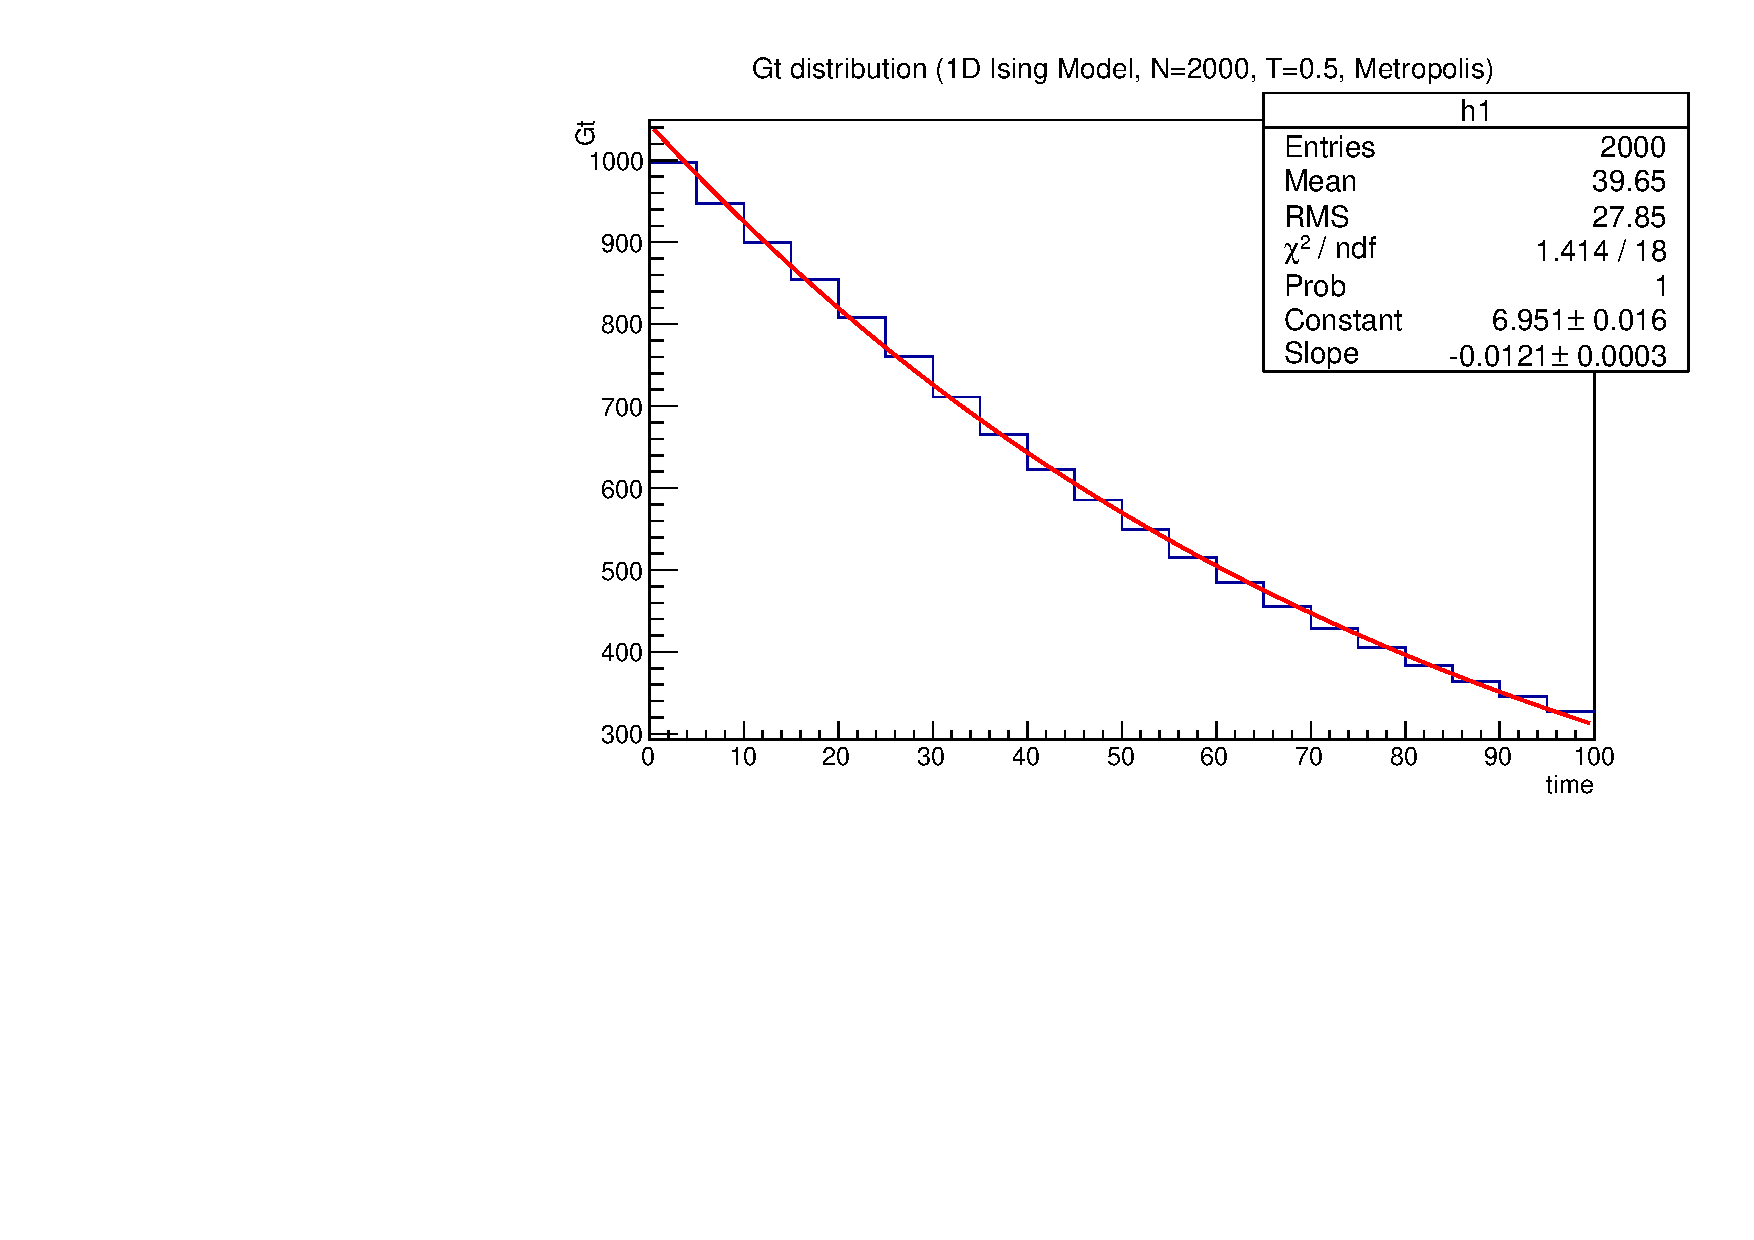
\includegraphics[scale=0.6]{IsingTestTCorr_Gt_1D_T05.pdf}
  \vspace{-0.05in}
   \caption[]{Gt vs time}   
  \label{gt_1d_t05}
\end{figure}



\begin{figure}[!ht]
\centering
  \subfigure{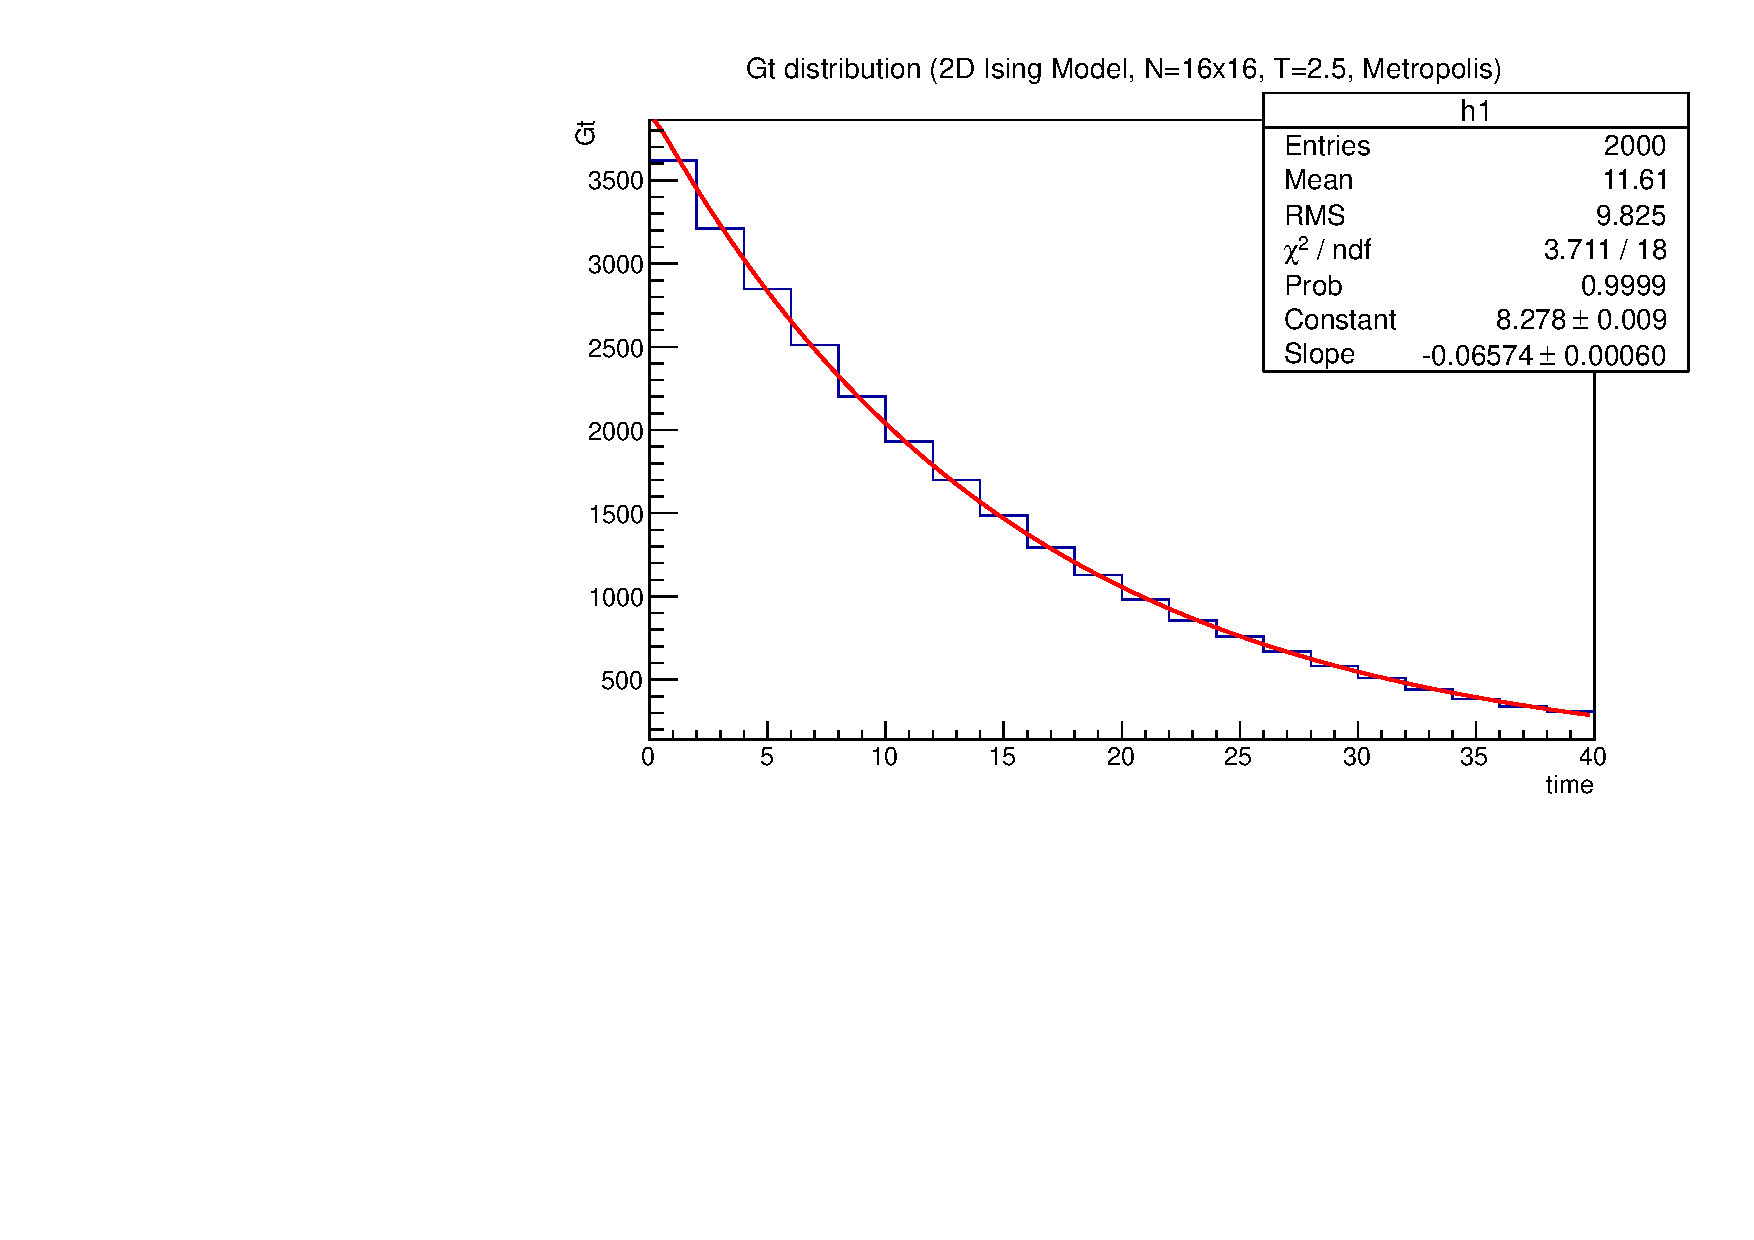
\includegraphics[scale=0.6]{IsingTestTCorr_Gt_2D_T25.pdf}}
  \hspace{-0.15in}
  \subfigure{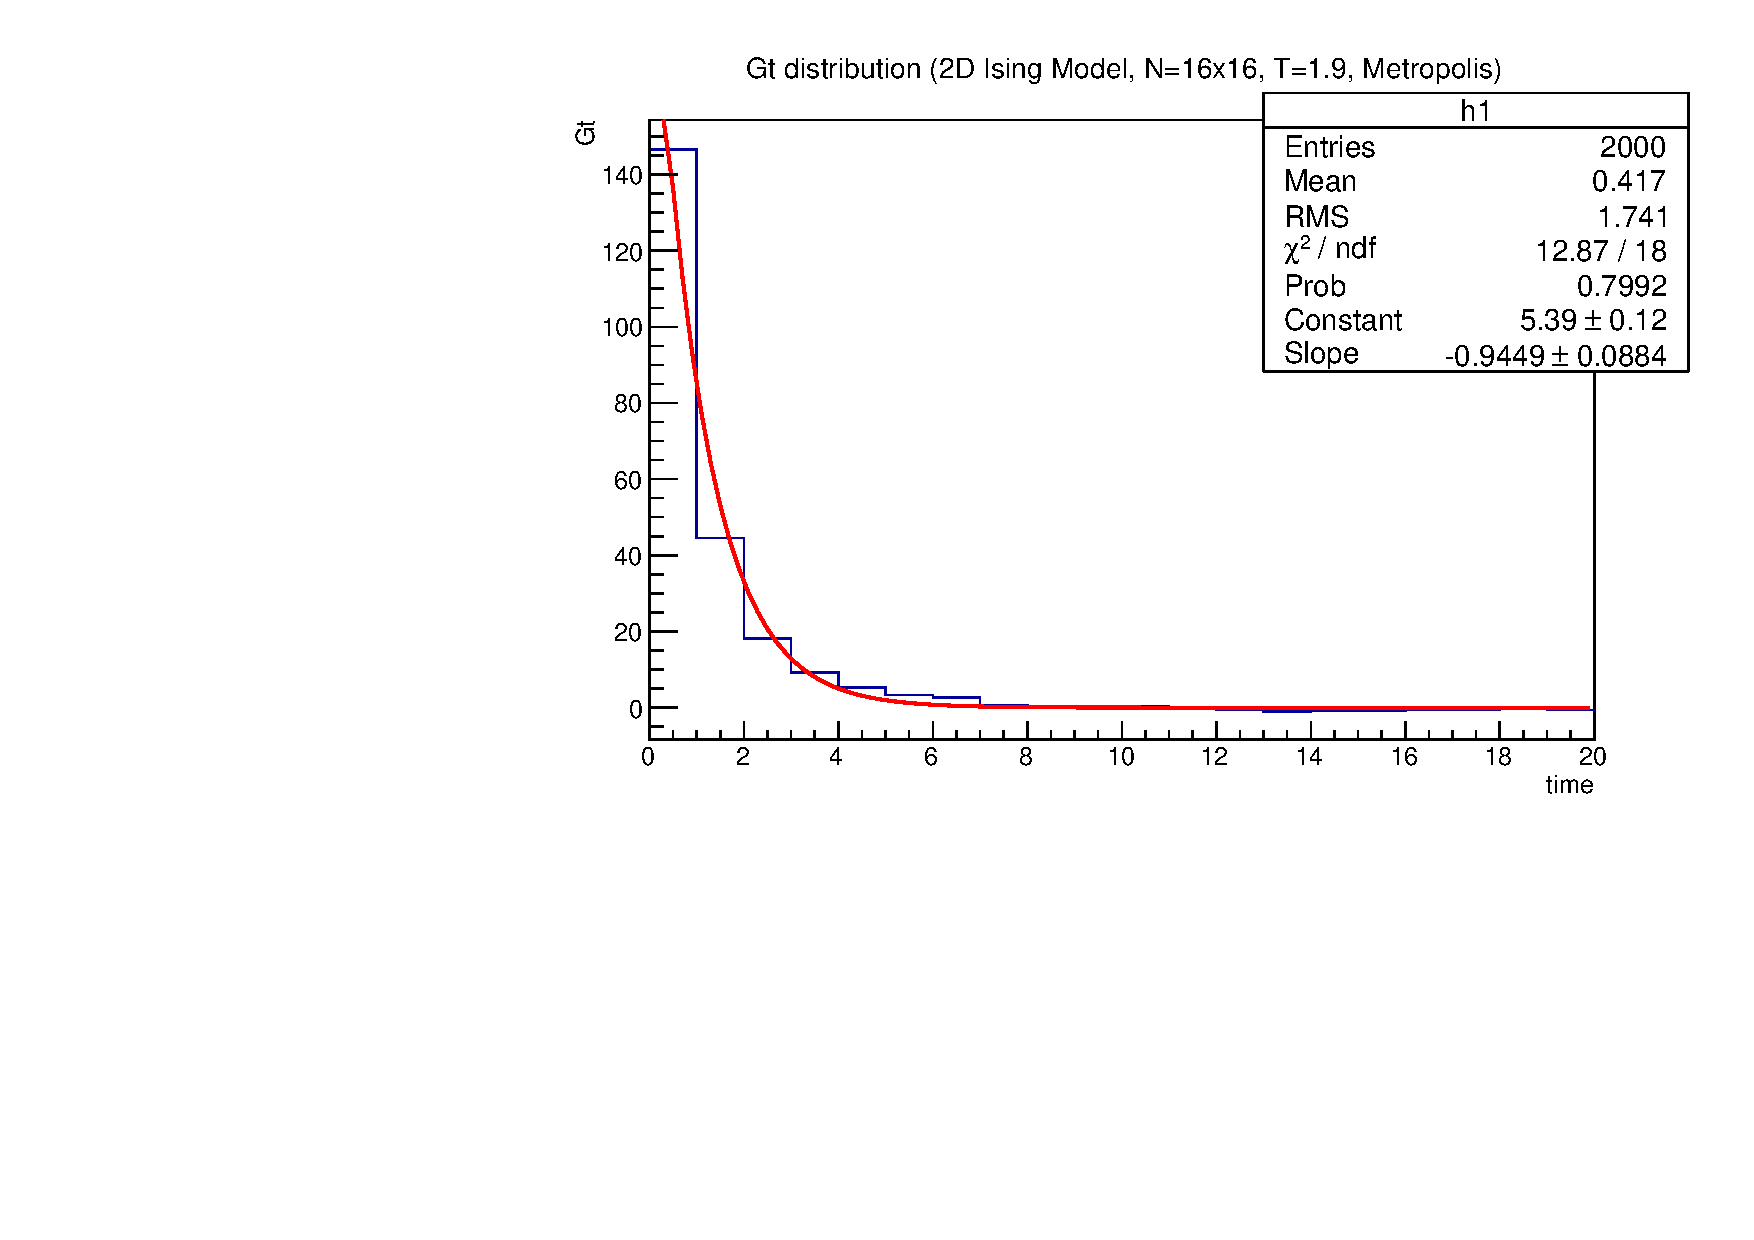
\includegraphics[scale=0.6]{IsingTestTCorr_Gt_2D_T19.pdf}} 
  \vspace{-0.05in}
   \caption[]{(top)...
   (bottom)...}   
  \label{gt_2d}
\end{figure}



\section{Relationship with critical exponents}
 The critical exponents of the transition in the Ising model are universal values and characterise the singular properties of physical quantities. 

\section{Summary}
...



%\clearpage
\bibliographystyle{unsrt}
\bibliography{common_project_mdyndal}







\end{document}
